%! Author = Saeid Yazdani
%! Date = 9/6/2024


\section{Combined Pre and Power Amplifiers Measurements}
\label{sec:combined-preamp-paamp-meas}

The power amplifier (PA95) was analyzed for \emph{Current Consumption},
\emph{Settling Time} and \emph{Stability}.

\subsection{PA95 Current Consumption}

The PA95 draws asymmetrical currents from the supplies where the current draw
from the positive rail is on average \SI{10}{\percent} higher than the
current drawn from the negative rail.
On average, both currents are between \SI{1.8}{\milli\ampere} to
\SI{2.8}{\milli\ampere}, about  \SI{200}{\micro\ampere} higher than the
specified value in the datasheet (\SI{1.6}{\milli\ampere} to
\SI{2.2}{\milli\ampere}) \autocite{apex:pa95}.

Although the difference in the current draw is small, asymmetrical current
draw can cause ripple or
noise on the floating power supplies and may
manifest as nonlinear behavior or as a DC offset on the output signal.
This offset can be measured during calibration and digitally compensated by
adjusting the set-point signal inside the FPGA.

\subsection{Stability Analysis}

Using the \ac{MCU} for controlling \emph{Dynamic Gain Array} of the power
amplifier, as presented in \autoref{fig:power-amplifier}, stability
of the combined output of the pre amplifier and power amplifier was evaluated
at different gain settings.

With $G<10$, oscillating waveforms were observed at the PA95 output for all
compensation values of the preamplifier as shown in
\autoref{fig:pa-lowgain-meas}.

\begin{figure}[htbp]
    \centering
    \begin{minipage}{0.48\textwidth}
        \centering
        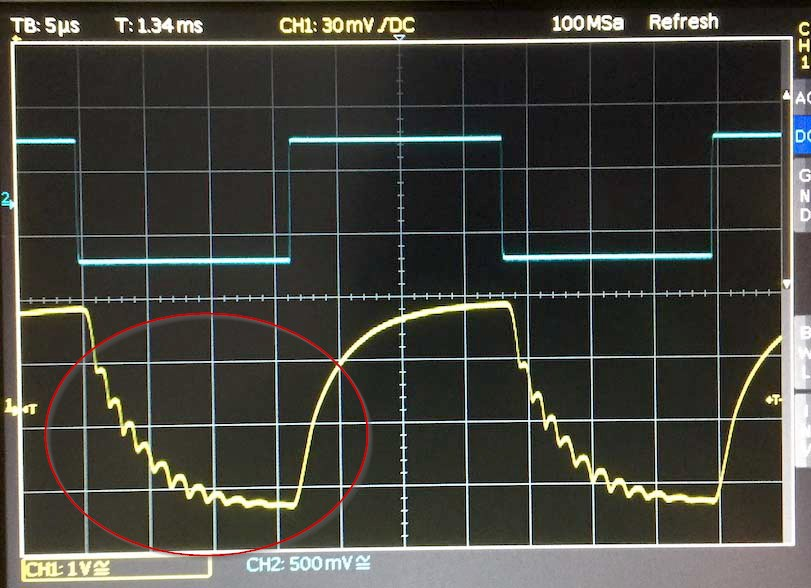
\includegraphics[width=\textwidth]{figures/tests/amptest/gain-lt10-precmp-low}
        \subcaption{Low Pre Amplifier B/W}
    \end{minipage}
    \hfill
    \begin{minipage}{0.47\textwidth}
        \centering
        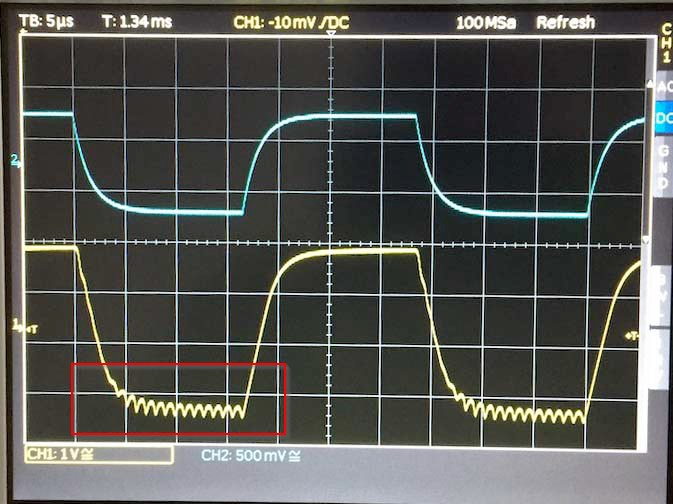
\includegraphics[width=\textwidth]{figures/tests/amptest/gain-lt10-precmp-high}
        \subcaption{High Pre Amplifier B/W}
    \end{minipage}
    \caption[Stability Measurement for $G < 10$ with Moderate B/W]{
        PA95 Stability Measurement for $G < 10$.
        \textbf{Blue Signal:} Pre Amplifier output.
        \textbf{Yellow Signal:} Power Amplifier output.
        \SI{5}{\micro\second} Timebase.
    }
    \label{fig:pa-lowgain-meas}
\end{figure}

Even with pre amplifier set to the maximum bandwidth, the oscillation still
appears on the falling edge as shown in \autoref{fig:pa-lowgain-pre-maxbw-meas}.

\begin{figure}[ht!]
    \centering
    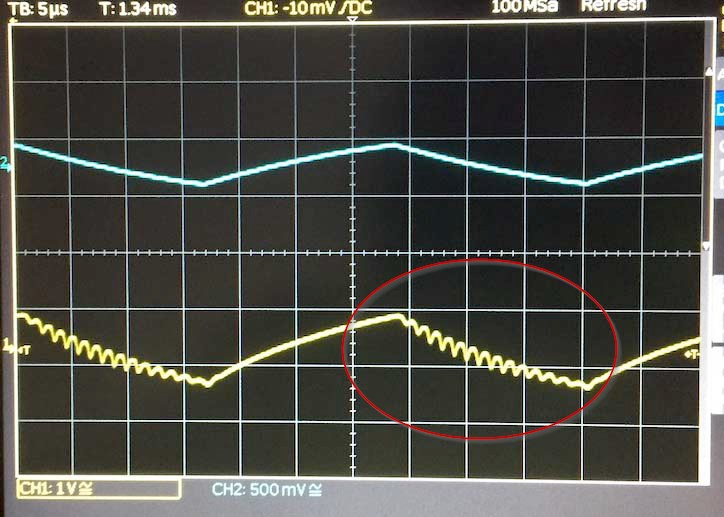
\includegraphics[width=0.52\textwidth]
    {figures/tests/amptest/gain-lt10-precmp-max}
    \caption[Stability Measurement for $G < 10$ with Max B/W]{
        Increasing the pre amplifier's bandwith to the maximum value does not
        remove the oscillation at the power amplifier's output.
        \SI{5}{\micro\second} Timebase.
    }
    \label{fig:pa-lowgain-pre-maxbw-meas}
\end{figure}

After thorough analysis, a few factors that can be attributed to this behavior
were identified:

\noindent\textbf{Lack of DC path:}
There was no DC path  in the local feedback of the pre amplifier as
depicted in \autoref{fig:test-preamp-isolation-circuit}.
A \acs{DC} path was added for stable operation as shown in
\autoref{fig:test-preamp-isolation-circuit-with-dc-path}.

\begin{figure}[h!]
    \centering
    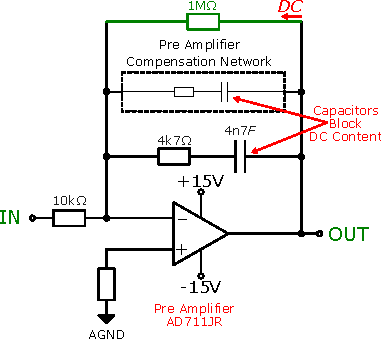
\includegraphics[width=0.6\textwidth]
    {figures/tests/preamp-test-circuit-with-dc-path}
    \caption[Pre-Amplifier With Added DC Path]{
        The capacitors in the series RC networks on the local feedback and
        compensation feedback block low-frequency DC content. Adding a
        resistor to the feedback path will allow DC content to flow.
    }
    \label{fig:test-preamp-isolation-circuit-with-dc-path}
\end{figure}

\noindent\textbf{Capacitance of relays in the feedback path:}
As stated before in \autoref{subsec:current-emasurement}, the compensation
network components and pre-scaler divider network are switched using analog
relays (\emph{OptoMOS} or \emph{PhotoMOS}) and the dynamic gain array uses
standard \acs{MOSFET}s which contribute to the total capacitance of the
control circuit.
The contribution of these stray capacitances
(up to \SI{50}{\pico\farad} per relay) must be taken into account in the
control loop processing.

\autoref {fig:gain-2dot4-with-stuff} shows the measurement repeated after
insertion of a resistor in the feedback path.
The oscillation at the falling edge is improved.

\begin{figure}[ht!]
    \centering
    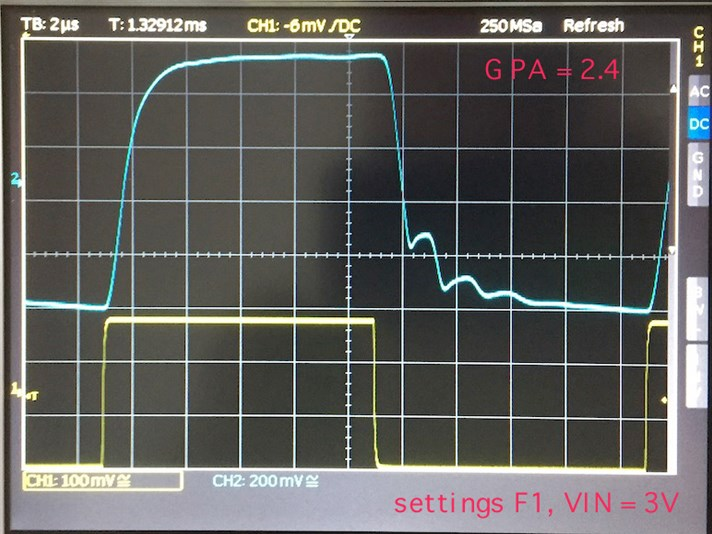
\includegraphics[width=0.52\textwidth]
    {figures/tests/amptest/gain-2dot4-with-stuff}
    \caption[Damped Oscillation]{
        The addition of a resistor for the DC path in the feedback has lowered the
        frequency content of the instability in the falling edge.
        \textbf{Blue Signal:} Power Amplifier output.
        \textbf{Yellow Signal:} Pre Amplifier output.
        \SI{5}{\micro\second} Timebase.
    }
    \label{fig:gain-2dot4-with-stuff}
\end{figure}
\subsection{Modification of PA95 Compensation Capacitor}
\label{subsec:modification-pa95-dedicated-comp}

High-gain or high-frequency operational amplifiers typically require
dedicated compensation capacitors to ensure stability and prevent unwanted
oscillations by design.
These capacitors are used for frequency compensation, which helps control the
amplifier's bandwidth and phase response.
This capacitor slows down the amplifier’s response to fast changes,
ensuring stable operation, especially in designs with feedback loops.

According to the power amplifier's datasheet \enquote{The PA95 is stable at
gains of 10 or more with
a compensation capacitor ($CC$) of 4.7pF mounted closely to pins 4 and 6 to prevent
spurious oscillation.
A compensation capacitor less than 4.7pF is not recommended}
\autocite{apex:pa95}.

The equivalent circuit presented in \autoref{fig:power-amplifier} shows this
capacitor connected to the $C_{COMP.}$ pins of the amplifier and actual value
is \SI{22}{\nano\farad}.
The placement on the \acs{PCB} layout is very close to the amplifier's pins
as depicted in \autoref{fig:pa95-cc-placement}.

\begin{figure}[t!]
    \centering
    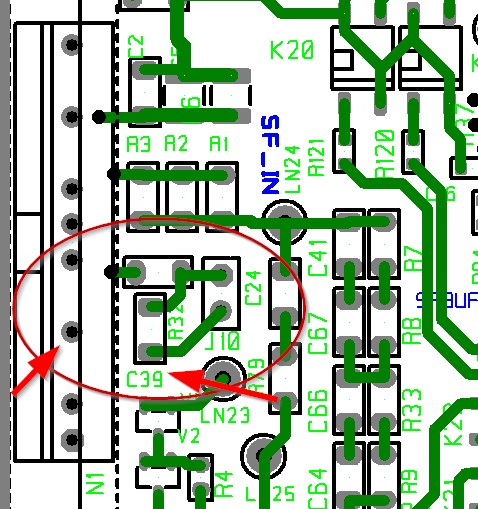
\includegraphics[width=0.6\textwidth]
    {figures/tests/amptest/pa95_cc_layout}
    \caption[PA95 $CC$ Placement]{
        The placement of the dedicated compensation capacitor for the power
        amplifier is optimal.
        \emph{N1} is the PA95 and \emph{C39} is the capacitor.
        A Series resistor \emph{R32} of \SI{10}{\ohm} is in series with the
        capacitor to dampen high-frequency oscillations.
        A Jumpr \emph{J10} is in parallel with \emph{C39}.
        \emph{J10} and \emph{R32} allow dropping in parallel and series
        capacitors to fine tune the compensation capacitor's final value.
    }
    \label{fig:pa95-cc-placement}
\end{figure}

A series of tests were carried out with different capacitor values, gain and
input voltages to verify the effect of the dedicated compensation capacitor on
power amplifier's output behavior.
This measurement results are presented in
\autoref{fig:pamp-cc-vs-gain} and verify that
a higher compensation capacitance for the power amplifier helps with reduction
of oscillation on the falling edge drastically.

\begin{figure}[htbp]
    \centering
    \captionsetup{font=footnotesize}
    \begin{minipage}{0.47\textwidth}
        \centering
        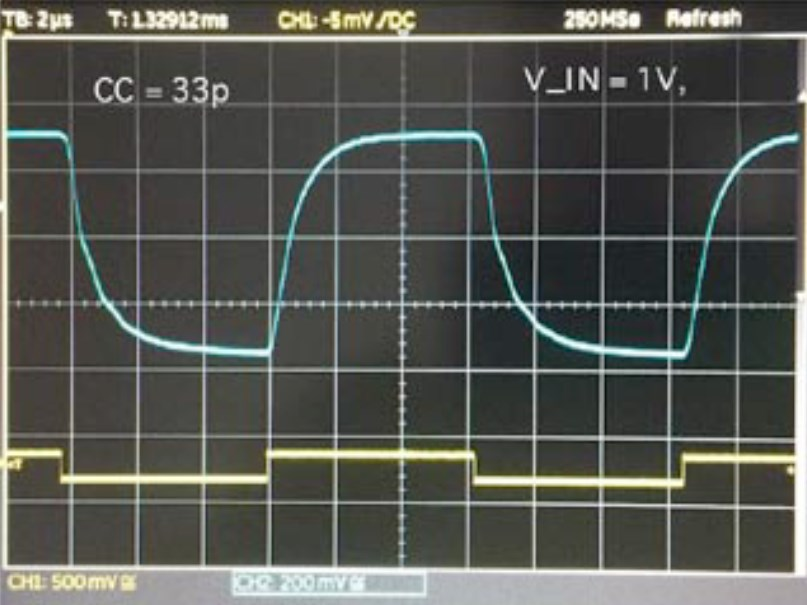
\includegraphics[width=\linewidth,height=0.18\textheight,keepaspectratio]{figures/tests/amptest/cc33-g2dot4-vin1}
        \subcaption{$G=2.4$, $C_C=33pF$ and $V_{IN}=1V$}\label{fig:cc33-g2dot4-vin1}
    \end{minipage}
    \hfill
    \begin{minipage}{0.47\textwidth}
        \centering
        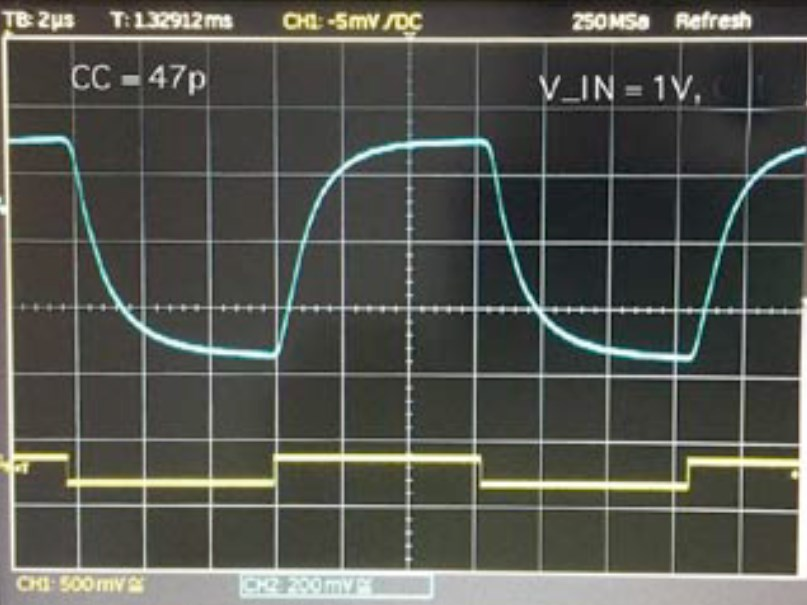
\includegraphics[width=\linewidth,height=0.18\textheight,keepaspectratio]{figures/tests/amptest/cc47-g2dot4-vin1}
        \subcaption{$G=2.4$, $C_C=47pF$ and $V_{IN}=1V$}\label{fig:cc47-g2dot4-vin1}
    \end{minipage}

    \vspace{0.12cm}

    \begin{minipage}{0.47\textwidth}
        \centering
        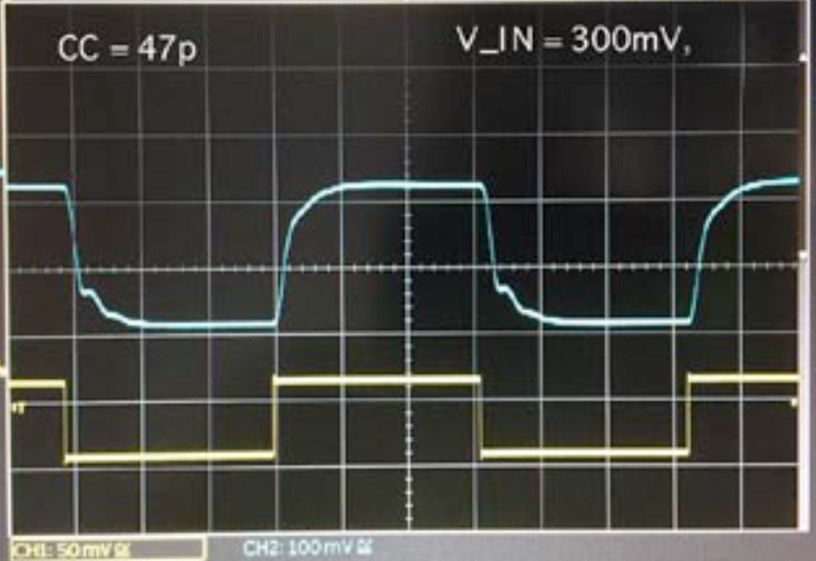
\includegraphics[width=\linewidth,height=0.18\textheight,keepaspectratio]{figures/tests/amptest/cc47-g2dot4-vin0dot300}
        \subcaption{$G=2.4$, $C_C=47pF$ and $V_{IN}=300mV$}\label{fig:cc47-g2dot4-vin0dot300}
    \end{minipage}
    \hfill
    \begin{minipage}{0.47\textwidth}
        \centering
        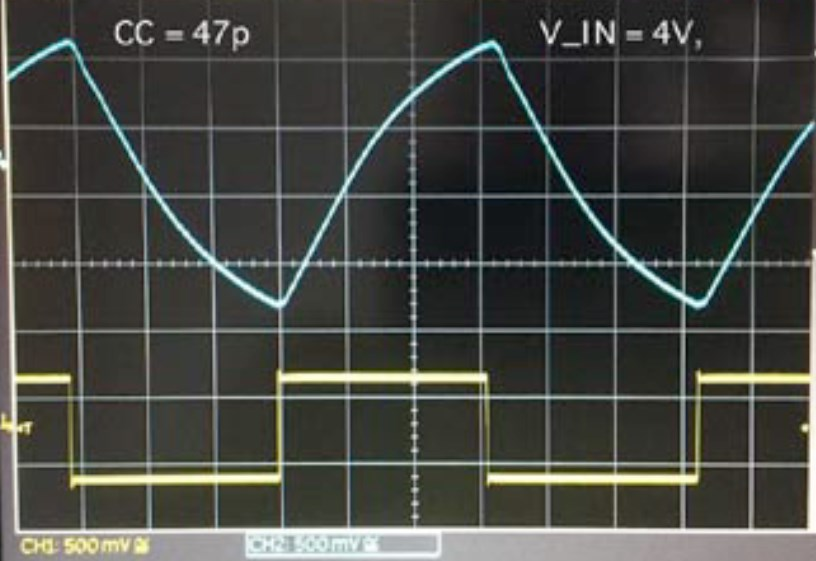
\includegraphics[width=\linewidth,height=0.18\textheight,keepaspectratio]{figures/tests/amptest/cc47-g2dot4-vin4}
        \subcaption{$G=2.4$, $C_C=47pF$ and $V_{IN}=4V$}\label{fig:cc47-g2dot4-vin4}
    \end{minipage}

    \vspace{0.12cm}

    \begin{minipage}{0.47\textwidth}
        \centering
        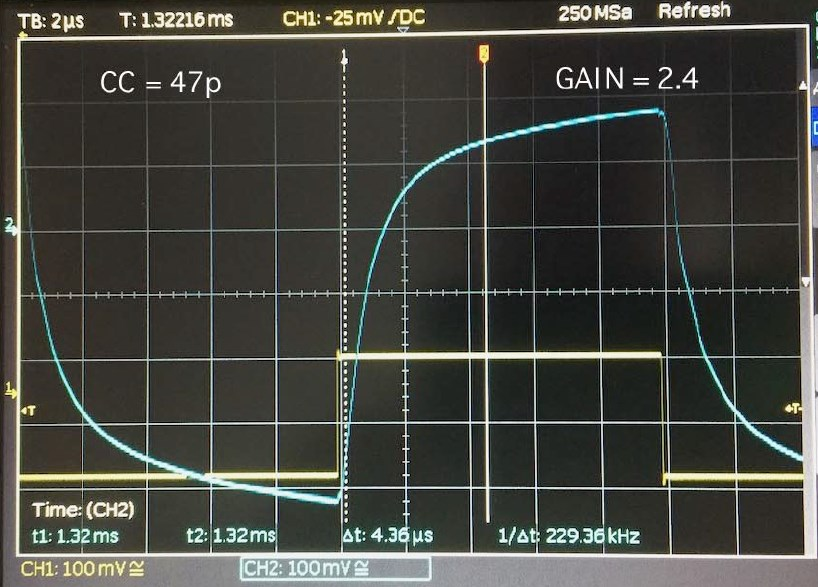
\includegraphics[width=\linewidth,height=0.18\textheight,keepaspectratio]{figures/tests/amptest/cc47-g2dot4-or10}
        \subcaption{$G=2.4$, $C_C=47pF$ and $V_{IN}=6V$}\label{fig:cc47-g2dot4-or10}
    \end{minipage}
    \hfill
    \begin{minipage}{0.47\textwidth}
        \centering
        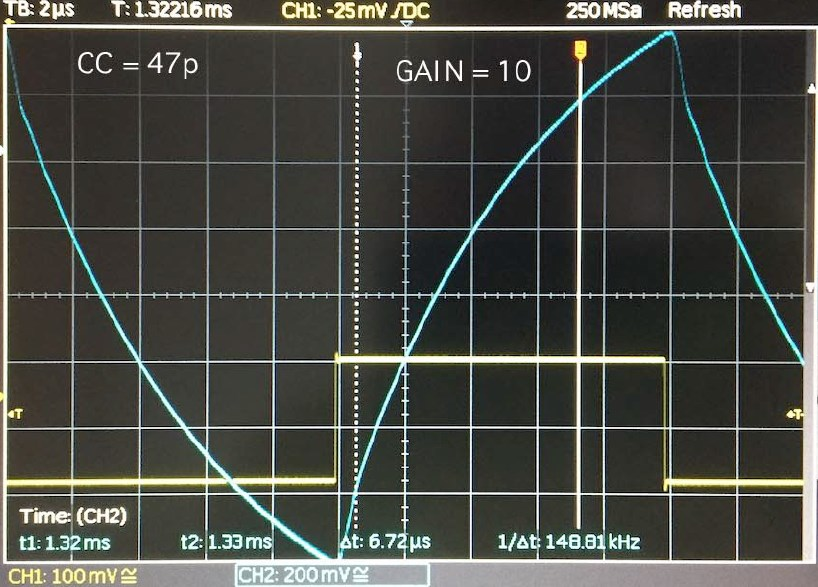
\includegraphics[width=\linewidth,height=0.18\textheight,keepaspectratio]{figures/tests/amptest/cc47-g10}
        \subcaption{$G=10$, $C_C=47pF$ and $V_{IN}=6V$}\label{fig:cc47-g10}
    \end{minipage}

    \caption[PA95 Dedicated Compensation Capacitor Effect]{
        Effects of PA95 dedicated $C_{COMP.}$ on the output based on
        various gain settings and input voltages.
        \textbf{Blue Signal:} Power Amplifier output.
        \textbf{Yellow Signal:} Pre Amplifier output.
        \SI{2}{\micro\second} Timebase.
    }
    \label{fig:pamp-cc-vs-gain}
\end{figure}

\subsection{Conclusion}
\label{subsec:amplifiers-conclusion}

The following points summarize the findings obtained by the measurements:
\begin{itemize}[topsep=8pt,itemsep=4pt,partopsep=4pt, parsep=4pt]
    \item The pre amplifier needs a DC feedback path.
    \item The divider stage requires a buffering amplifier for compensation.
    \item The power amplifier's higher gains result in a limited slew rate.

    \item The power amplifier's dedicated compensation capacitor must be
    increased.
    \item Swing range of the pre amplifier needs adjustment.
\end{itemize}

\clearpage
